\begin{figure}[tbp]
% \vskip -.1in
    \centering
    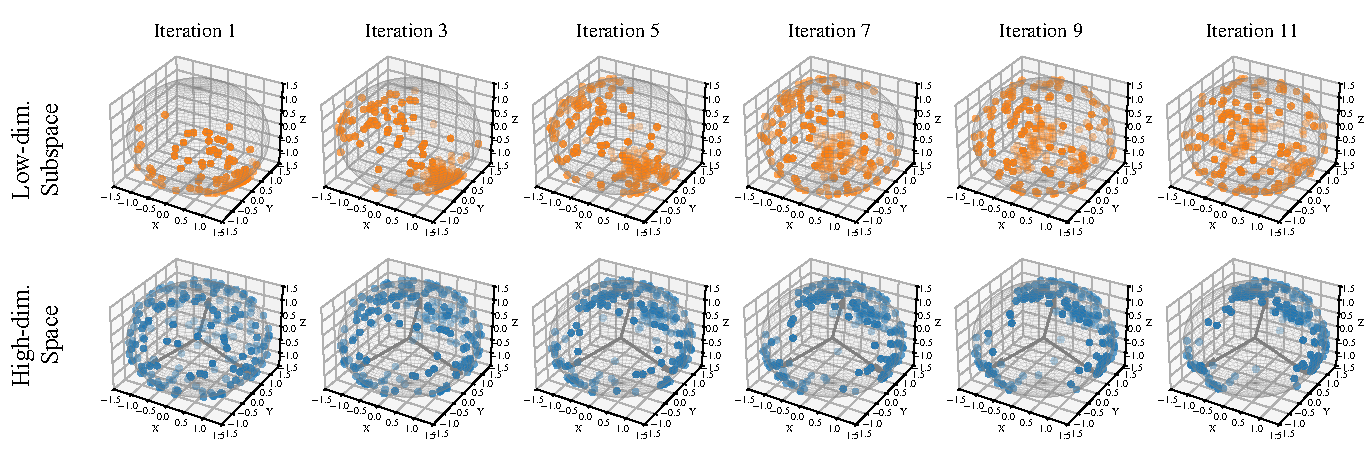
\includegraphics[width=\linewidth]{figures/figure1_iclr2026.pdf} 
        % \vskip -.2in
    \caption{Evolution of tokens in the forward pass. \emph{Top}: Tokens projected onto subspaces are progressively separated on the \textbf{low-dimensional} hypersphere. \emph{Bottom}: Tokens gradually align with anchor vectors in the \textbf{high-dimensional} hypersphere. Visualization is carried out in three-dimensional space for illustrative purposes.}
    \label{fig:dynamics_on_hypersphere}
    % \vskip -.2in
\end{figure}
To answer the introductory question, we conjecture that effective representations should exhibit two complementary properties: \textbf{semantic alignment} in a high-dimensional space and \textbf{distributional uniformity} in a low-dimensional subspace. This dual perspective reflects the balance of \emph{mode seeking} and \emph{mass covering}—terms we use to characterize the interplay between information preservation and entropy collapse prevention in representation learning. Figure~\ref{fig:dynamics_on_hypersphere} shows an illustrative example.
% \subsection{Instantiation}

We formalize this conceptualization under maximum likelihood estimation. Specifically, we instantiate the forward dynamics as an optimization over a token-level vector $\vx$ balancing two terms:
\begin{equation}
\label{eq:mle ultimate form}
\min_{\vx} ~\sum_{h=1}^H \underbrace{\KL \left( p(\vz) \Vert p_\phi(\vz^h \mid \vx) \right)}_{\text{uniformity}} \underbrace{- \log p_\theta(\vx)}_{\text{alignment}},
\end{equation}
where $\vz^h$ represents low-dimensional projections of the high-dimensional representation $\vx$. 

The first term encourages the projections $\vz^h$ to approximate a prior uniform distribution $p(\vz)$ on a hypersphere, thus maximizing entropy and mitigating representational collapse. The second term promotes alignment between $\vx$ and mean directions, which can be modeled using von Mises–Fisher distributions. A detailed justification and interpretation of this objective is provided in Appendix~\ref{section:justification}.

This objective resonates with but differs from the contrastive learning objective that unifies alignment and uniformity in a shared latent space \citep{wang2020understanding}. Our work instead takes on an energy view to quantify these two key ingredients into optimizable functions of $\vx$ that can induce Transformer architectures.